\subsection{Implementation}

Formålet med dette afsnit er at give en beskrivelse af programmets opbygning og struktur, samt ved brug af kodeeksempler at illustrere hvordan der gøres brug af den tidligere beskrevet teori til at lave programmet. I afsnittet vil der kun fremgå udvalgte kodeeksempler, men hele programmet kan findes i bilag. 

\subsubsection{Programbeskrivelse}

Programmet er udarbejdet som et suplement til hjemmesider som sælger lamper. Formålet med programmet er som beskrevet tidligere, at hjælpe kunderne med at visualisere lampers belysning. Programmet ligger fokus på realitsk visualisering af lys fra lamper, samt muligheden for at ændre pærens farvetemperatur.
Nedenstående figur viser et billede af renderingen fra det færdige program

\#Indsæt rendering fra det færdige program
\#nærmere beskrivelse af billede

\subsubsection{Programmets opbygning}

Programmet er opbygget efter desginprincippet "top-down programmering". Princippet går ud på at dele programmet og i mindre dele, og derefter løse de mindre dele i hver deres funktion. Funktionerne samles i main, som kun bruges til kommunikation med brugeren. 
\ref{fig:topdown} viser tankegangen bag top-down programmering, hvor de enkelte problemer deles op og løses som delproblemer. 

\begin{figure}[H]
    \centering
    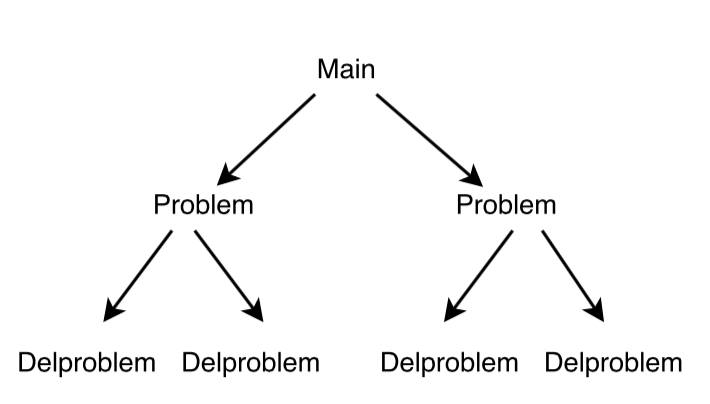
\includegraphics[width=10cm]{topdown}
    \caption{Tankegangen bag top-down programmering.}
    \label{fig:topdown}
\end{figure}

Som en del af vores top-down fremgangsmåde har vi struktureret opgaven i header-filer som blandt andet indeholder prototyper og structs. Header-filerne hjælper os med, at få bedre overblik over koden. 

\subsubsection{Vektorregning}

En vigtig del af vores raytracer består af vektorregning. For at regne med vektorer, er det først nødvendigt at lave en struct vector, der fortæller programmet hvad en vektor består af. Som set på programmet (skriv nummer på program) kan det ses at en vektor består af tre koordinater, x, y og z. 

\begin{lstlisting}[language=C, caption=Vektorprototyper og struct]

typedef struct _vector {
    double x,y,z;
} Vector;

Vector vector_add(Vector v1, Vector v2);
Vector vector_subtract(Vector v1, Vector v2);
Vector vector_scale(Vector v, double s);
double vector_dot(Vector v1, Vector v2);
double vector_norm(Vector v);
Vector vector_normalize(Vector v);
double vector_angle_between(Vector v1, Vector v2);
Vector vector_cross(Vector v1, Vector v2);
Vector vector_rotate_around_z(Vector v, double angle);
Vector vector_rotate_around_x(Vector v, double angle);

\end{lstlisting}

Et eksempel på én af vores vektorudregninger er vector_add. Denne funktion adderer to vektorer, som det ses på (program nr bla). Her kan man se, at ved addition af to vektorer, adderer man x-koordinaterne med hinanden og det samme gælder for y- og z-koordinaterne. Resultatet vil også være en vektor.

\begin{lstlisting}[language=C, caption=vector add]

Vector vector_add(Vector v1, Vector v2) {
  return (Vector){v1.x + v2.x, v1.y + v2.y, v1.z + v2.z};
}

\end{lstlisting}

Et andet eksempel på en vektorudregning, vi gør brug af, er skalarproduktet af to vektorer. Det er vigtigt at kende skalarproduktet, da det benyttes i vector_norm for at finde længden af to vektorer og i vector_angle_between for at finde vinklen mellem to vektorer. Herunder kan det ses, at skalarproduktet simpelt findes ved at gange de tilsvarende koordinater med hinanden.

\begin{lstlisting}[language=C, caption=vector dot]

double vector_dot (Vector v1, Vector v2) {
  return v1.x * v2.x + v1.y * v2.y + v1.z * v2.z;
}
\end{lstlisting}

\begin{enumerate}

  \item vector add adderer to vektorer.
  \item vector subtract –subtraherer to vektorer.
  \item vector scale skalerer en given vektor.
  \item vector dot prikker to vektorer sammen. Resultat bruges i vector norm og vector angle between.
  \item vector norm finder længden af to vektorer.
  \item vector normalize normaliserer vektoren (ændrer længden til 1), så man kun har retningen af vektoren tilbage.
  \item vector angle between finder vinklen mellem to vektorer.
  \item vector cross Udregner krydsproduktet og finder dermed normalvektoren.
  \item vector rotate around z og vector rotate around x roterer en given vektor omkring hhv. z- eller x-aksen.

\end{enumerate}